\documentclass{standalone}
\usepackage{tikz}
\begin{document}
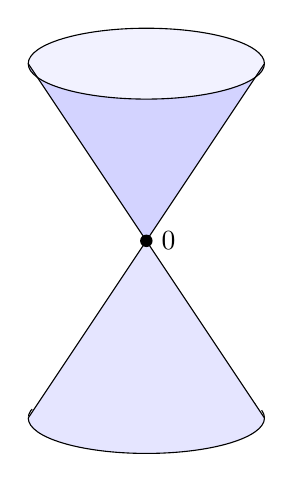
\begin{tikzpicture}[scale=1.5]
    % Back half of lower cone
    \draw[dashed] (1,-1.5) arc (0:180:1 and 0.3);
    
    % Lower cone shading and front outline
    \fill[blue!10] (0,0) -- (-1,-1.5) arc (180:360:1 and 0.3) -- cycle;
    \draw (-1,-1.5) arc (180:360:1 and 0.3);
    \draw (-1,-1.5) -- (0,0) -- (1,-1.5);
    
    % Upper cone inside (back half)
    \fill[blue!5] (0,0) -- (-1,1.5) arc (180:0:1 and 0.3) -- cycle;
    
    % Upper cone front shading
    \fill[blue!20, opacity=0.8] (0,0) -- (-1,1.5) arc (180:360:1 and 0.3) -- cycle;
    
    % Upper cone outlines
    \draw (0,1.5) ellipse (1 and 0.3);
    \draw (-1,1.5) -- (0,0) -- (1,1.5);
    
    % Origin
    \fill (0,0) circle (1.5pt) node[right=2pt] {$0$};
\end{tikzpicture}
\end{document}
